\begin{flushleft}
    \huge
    \section{Evaluation}
    \vspace{0.1cm}

    \large
    \subsection{Evaluation of Objectives}
        \vspace{0.2cm}
        In this section, I will evaluate my overarching objectives I set out to complete.
        \vspace{0.2cm}

        \subsubsection{Reading user inputted data}
            \vspace{0.2cm}
            The user can input the parameters through a json file, and these parameters are checked against a range file to check they are within
            the specified size. All of the parameters are read correctly and utilised within the Program. \\
            \vspace{0.2cm}
            The Machine Learning Data is read from .dqn files. The Learning is resumed from where it was saved from with all the Weights and
            Biases intact. \\

            \vspace{0.5cm}    
        \subsubsection{Generating the Environment}
            \vspace{0.2cm}
            At the start of the program an instance of World Class is created and the Generate methods are invoked. These methods utilise Perlin
            Noise and Poisson Disc Sampling. The Terrain values are stored in a 2d list of Tile Objects which store the Height, Type and Colour data
            for each Tile. The Poisson Disc Sampling Generates a list of points which Trees are then generated at those positions. The Width
            of the world and Tile colours are determined by the Input Parameters. \\

            \vspace{0.5cm}    
        \subsubsection{Displaying the world to a Pygame Window}
            \vspace{0.2cm}
            Upon generating the Map Data the Terrain is displayed in a grid to the Pygame Window, it is represented as a grid of tiles of the pixel 
            width loaded in by the Inputted Parameters. The Agent and Enemies are Drawn at their according positions, taking up entire Tile. If Debug
            mode is enabled, a representation of the Neural Network will be displayed on the right hand side of the window. \\

            \vspace{0.5cm}   
        \subsubsection{Simple Agent with a set of Actions}
            \vspace{0.2cm}
            An Agent can be created as an object and works along side the Dual Neural Network Object to enable interactions between the environment and
            the Network. The Agent can collect the surroundng Tile Data using the \textbf{GetTileVector} Method, this can then be converted into the
            Networks Input Vector using the \textbf{TileVectorPostProcess} Method. There exists Methods to Take a given Action, normally outputted by
            the Network. Along with Methods to Calculate Reward for an Action given a State, or the Maximum Possible Reward Given a State. \\
            \vspace{0.2cm}
            There also exists Methods to Reset the Agent to its default values. Along with Determining the Agents Spawn Position when given a WorldMap
            Object. \\

            \vspace{0.5cm}   
        \subsubsection{Matrix Class with Standard Operations}
            \vspace{0.2cm}
            A Matrix can be created using 3 different methods. First using a Tuple of Integers, a new Matrix will be created of that size, with initialised
            0 values. Second using a prexisting 2d list of values, a new Matrix will be created with these dimensions and values. Thirdly a 1d list of
            values can be used to create a 1 wide Vector of values, where it reads each value into the 1st position of each row. \\
            \vspace{0.2cm}
            All standard operations for the Matrix Object are implemented using Operator Overloading to make code less bloated. All are written 
            efficiently utilising minimum complexity algorithms. Addition can be carried out utilising the $+$ Operator. Subtraction can be carried out
            utilising the $-$ Operator. Multiplication and Scalar Multiplication are both carried out utilising the $*$ Operator. Power Operation is
            carried out utilising the $\string^$ operator. A Matrix can be converted to a Formatted String implicitly by using it in a string context. \\
            \vspace{0.2cm}
            All Matrice Operations have appropriate Exceptions with descriptive Error Messages. They will throw errors when incorrect Data is provided to
            the specified Operation. \\

            \vspace{0.5cm}   
        \subsubsection{Creation of a Reinforcement Learning Model}
            \vspace{0.2cm}
            A Dual Neural Network can be created as an object, which stores two Neural Network Objects, Main and Target. The Dual Neural Network
            contains the Primary Method \textbf{Step} which invokes a Series of Lower Level Methods to perform a singular Time Step. The Neural 
            Network Object store a List of Layers Objects which are dynamically created from the Input Parameters. Each Layer contains a Weight 
            Matrix, Bias Vector, and Output Vector. The Lowest Level methods for Forward and Back Propagation are contained within the Layer Object. \\
            \vspace{0.2cm}
            First Forward Propagation occurs on the Main and Target Network. Then results of the Main Network are taken to choose the action for the Agent. 
            Epsilon Greedy is implemented to determine whether to choose the random or predicted result. This Action is then fed to the Agent, along with 
            calculating the reward for that Action. The Loss of the Main Network is then calculated using a modified Bellman Equation for Dual Neural 
            Networks. This Loss is used for Back Propagating the Main Neural Network. The Main Networks Weights are copied to the Target Network
            every specified ammount of steps. Every specified ammount of steps, Experience Replay is performed to learn from past experiences again. \\
            \vspace{0.2cm}
            The combination of these steps form a functional Dual Neural Network utilising a Reinforcement Learning Model. \\

            \vspace{0.5cm}   
        \subsubsection{Creation of a Data Logger}
            \vspace{0.2cm}
            A Data Logger Class can be used to Log and Store Data Points at various parts of the Program. Each Data Point is stored as a Tuple of Values
            as part of a .data file. These files are stored as Binary Files, and are Read into the Program upon launch. \\
            \vspace{0.2cm}
            As part of the Data Logger you can sort points utilising a Heap Sort to sort through Data. \\

            \vspace{0.5cm}   

        \vspace{0.5cm}
    \subsection{Analysis of Training Data}
        I found that the Network is sensitive to its reward structure and Network architecture. When the Reward Structure has an action which
        gains 0 but also loses 0 reward, the Back Propagation will minimise the Network into purely taking this action. An example of this
        is when "Noop" or the Null Action is enabled. This ended up in the graph just flatlining towards 0 average loss, where the Network
        only took the null action 99\% of the time. 

        \begin{figure}[H]
            \centering
            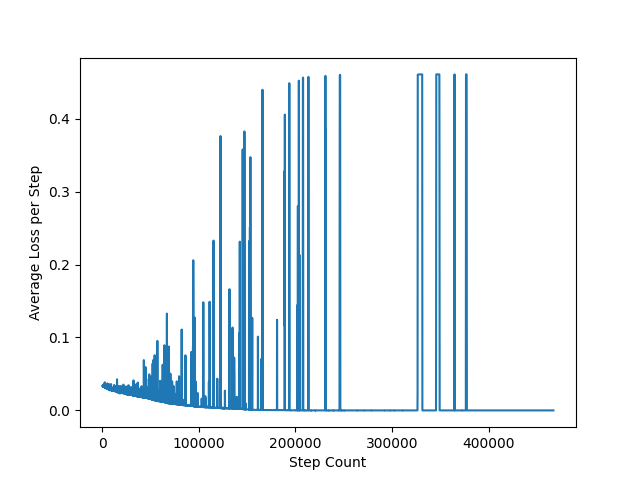
\includegraphics[width=12cm]{Images/Evaluation/NullActionFlatline.png}
            \caption*{Neural Network flatlining towards 0 loss by only picking "Noop"}
            \caption*{Large network architecture with 49 Input Nodes} 
            \caption*{Enemies Disabled}
        \end{figure}

        I am unsure as to what the spikes are, I believe it is due to instabilities in the training architecture. Following on from this failed attempt
        to train the Network, I removed Noop from the action set. This led to overall weird results, the baseline Loss trends down, but doesnt manage to
        overall minimise it. I believe this is a sign that the simulation is too complex for the Network architecture to solve. 

        \begin{figure}[H]
            \centering
            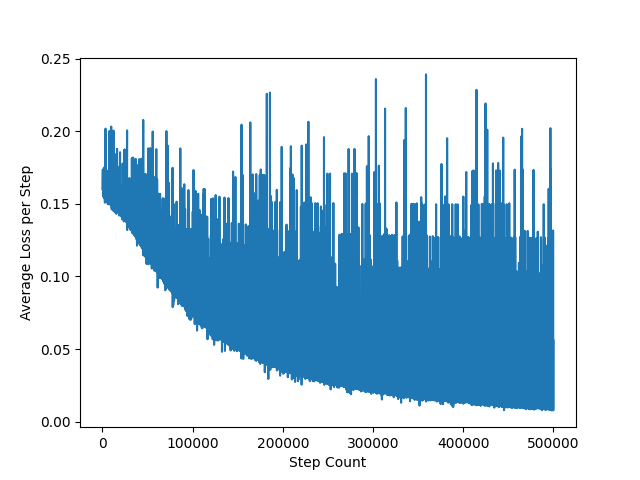
\includegraphics[width=12cm]{Images/Evaluation/AttemptedMinimiseLargeNetwork.png}
            \caption*{Neural Network attempts to minimise network but fails to solve the simulation}
            \caption*{Large network architecture with 49 Input Nodes} 
            \caption*{Enemies Disabled, Attack and Noop action disabled}
        \end{figure}

        I then enabled the enemies with the same Network architecture, this led to different results. The Network clearly places a signifcance on their
        existence, but fails to overcome them as a problem. I observed during this training session that the Agent does manage to kill enemies sometimes.
        but fails to do this consistently. I believe this might be due to the high sensory input.

        \begin{figure}[H]
            \centering
            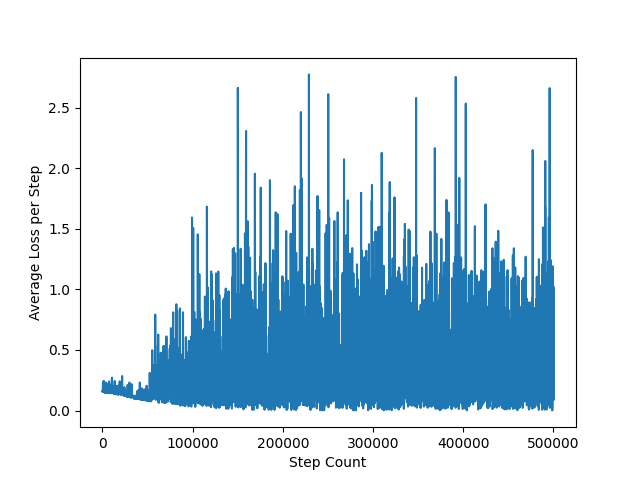
\includegraphics[width=12cm]{Images/Evaluation/EnemiesEnabled.png}
            \caption*{Neural Network struggles with Enemies}
            \caption*{Large network architecture with 49 Input Nodes} 
            \caption*{Noop action disabled}
        \end{figure}

        I also attempted training using different Network architectures, this led to much better results compared to the previous training session with 49 Inputs.
        This as stated previously may be due to the high sensory input of a larger Network. I think the 25 Input Network performs ever so slightly better than
        the 9 Input, but this may only be due to random chance.

        \begin{figure}[H]
            \centering
            \subfloat[\centering 25 Input Nodes]{{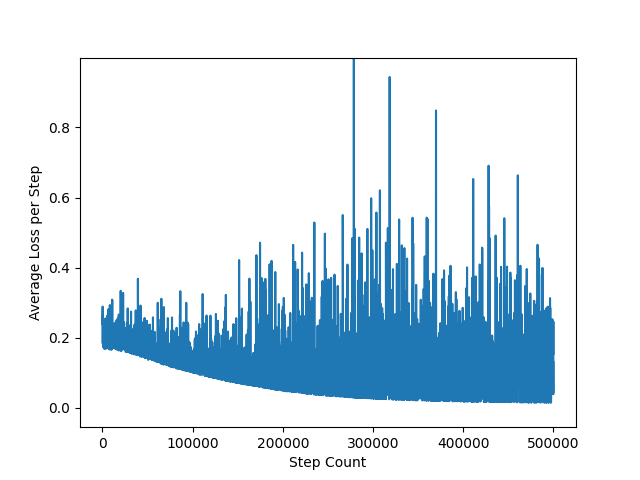
\includegraphics[width=7cm]{Images/Evaluation/25InputNetwork.png}}}
            \qquad
            \subfloat[\centering 9 Input Nodes]{{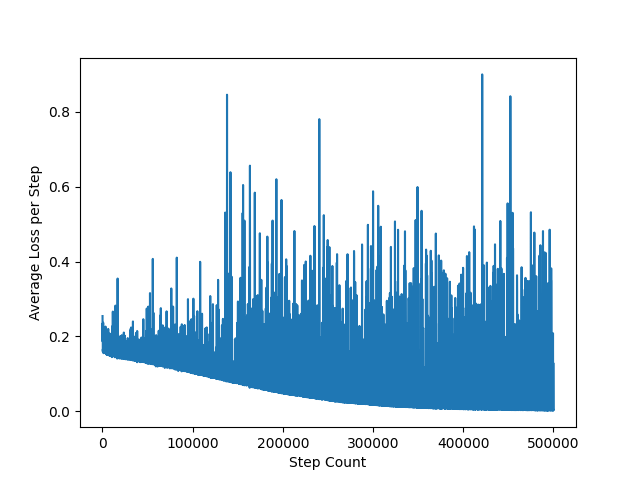
\includegraphics[width=7cm]{Images/Evaluation/9InputNetwork.png}}}
        \end{figure}

        I then chose the best performing Network out of the 3 I tested, which has 25 Inputs, and tried it with all the Activation Functions I've implemented. Previously
        I had just been using the standard Sigmoid Activation funtion. This is an attempt to find the best possible Network $\rightleftharpoons$ Activation Combination.

        \begin{figure}[H]
            \centering
            \subfloat[\centering Sigmoid Activation Function]{{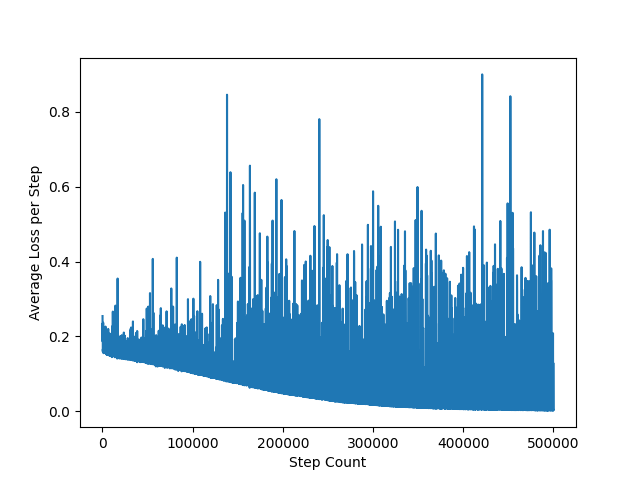
\includegraphics[width=8cm]{Images/Evaluation/9InputNetwork.png}}}
            \qquad
            \subfloat[\centering TanH Activation Function]{{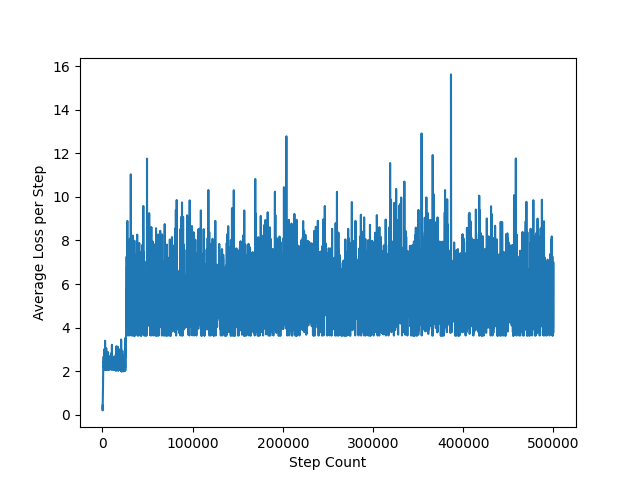
\includegraphics[width=8cm]{Images/Evaluation/9InputNetworkTanH.png}}}
            \qquad
            \subfloat[\centering ReLu Activation Function]{{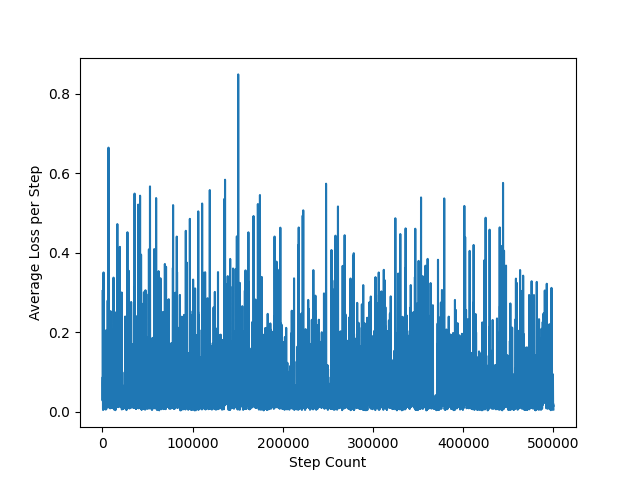
\includegraphics[width=8cm]{Images/Evaluation/9InputNetworkReLu.png}}}
            \qquad
            \subfloat[\centering Leaky ReLu Activation Function]{{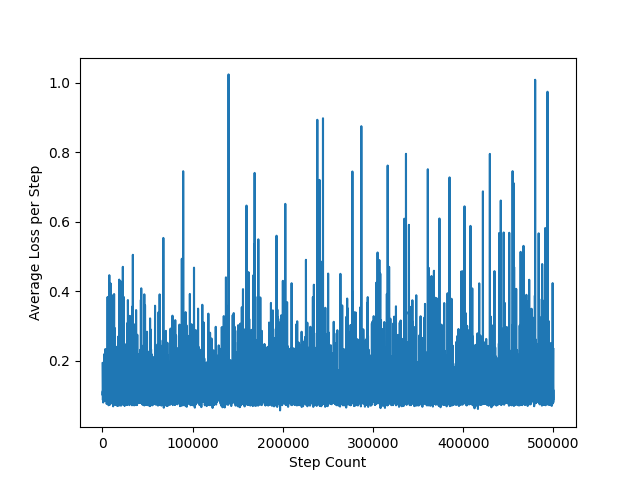
\includegraphics[width=8cm]{Images/Evaluation/9InputNetworkLeakyReLu.png}}}
        \end{figure}

        As shown above Sigmoid is clearly the best Activation Function to use for the problem. TanH exhibits weird behaviour which I can't explain. 
        ReLu and Leaky ReLu preform similarly, with Leaky ReLu being slightly better but both may as well be random. Leaving us with the best Network 
        Architecture with a layer structure of $[25,32,16,8,6]$, utilising the Sigmoid Activation Function. \\
        \vspace{0.2cm}
        In an attempt to reduce the complexity of the simulation I created, I altered the simulation slightly. I turned off the Enemies movement,
        this was an attempt to reduce the difficulty of the problem for the Agent. I also spawned 30 rather than 5 enemies at the start of a created
        world. This resulted in somewhat better results when compared to previous results, the baseline loss minimises towards 0 quicker. This is 
        definitely because the Network finds static threats easier to deal with. I also noticed in the previous test that the Agent didn't appear 
        to have a problem avoiding the Static Enemies, so I kept this for the next test.

        \begin{figure}[H]
            \centering
            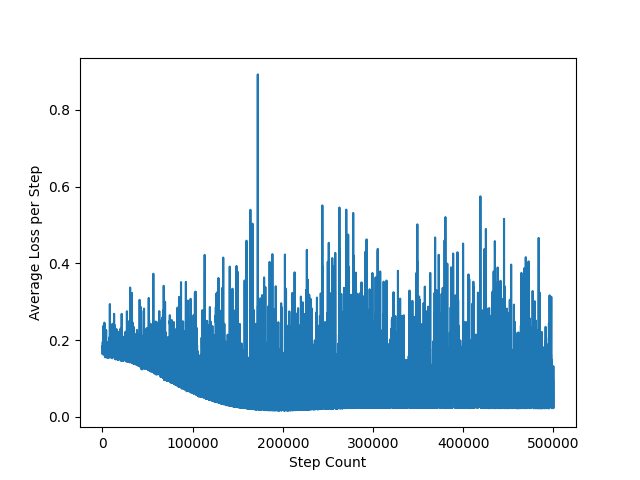
\includegraphics[width=12cm]{Images/Evaluation/StaticEnemiesExtra.png}
            \caption*{Altered Simulation Data using Static Enemies}
            \caption*{25 Input Nodes}
        \end{figure}

        This next test involved me changing the Colour of the Water to the same colour as the Enemies. I figured that this would improve the Networks
        Ability to determine what is a threat to its Survival. Instead of having to form a relationship between two colours, it was only one. This
        performed quite well in comparison to previous tests. The overall average loss is less than every other test, and shows that the Network is 
        actually capable of determining relationships between the input values and correct outputs.

        \begin{figure}[H]
            \centering
            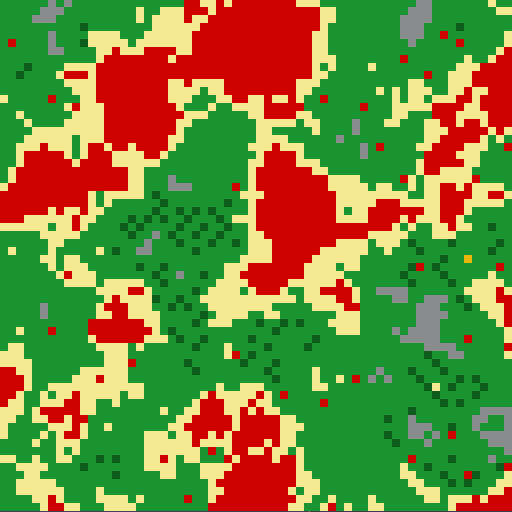
\includegraphics[width=8cm]{Images/Evaluation/RedWaterTest.PNG}
            \caption*{Altered Simulation using Static Enemies and Red Water}
            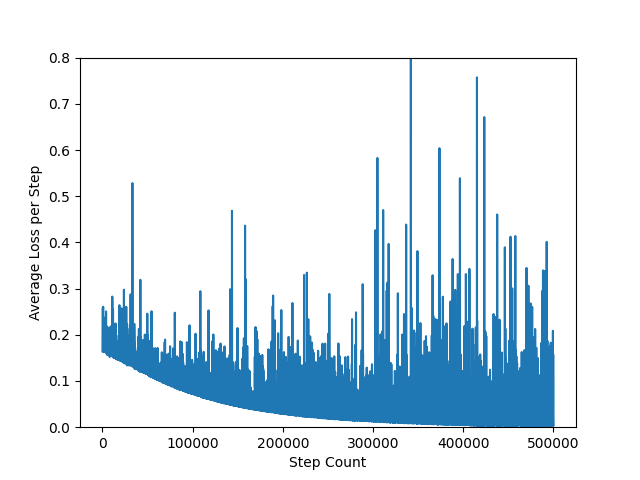
\includegraphics[width=12cm]{Images/Evaluation/RedWaterStaticExtra.png}
            \caption*{Simulation Data}
            \caption*{25 Input Nodes}
        \end{figure}

    \pagebreak
    \subsection{Answering the Proposed Questions}
        \vspace{0.2cm}
        As part of my Machine Learning Investigation I proposed the Question:

        \vspace{0.3cm}\begin{center}
        \textbf{Can I develop a Machine Learning Algorithm to survive in a pseudorandom, open-world environment?}
        \end{center}\vspace{0.3cm}

        I aimed to answer this question by designing and creating a Deep Reinforcement Learning Model utilising a Deep Neural Network, along 
        with designing a Simple Simulation for a Machine Learning Agent to survive in. \\
        \vspace{0.2cm}
        With the Machine Learning Model I implemented, the Agent was unable to fully solve the simulation. After being trained to 500000
        steps with multiple different layer structures and parameters, it fails to achieve a true solution to the problem at any given time step.
        The Average Loss of of the Network for most of my tests trends downwards, but still remains highly innacurate. The graphed data shows
        that the Average Loss (Plotted per 100 Steps) constantly peaks and drops back down to the baseline. This baseline for most of the tests
        I performed trends downwards as a curve. All the Tests Data is shown above. \\
        \vspace{0.2cm}
        Because the implemented algorithm has not managed to fully solve the problem, I have answered the sub-questions I outlined in my 
        \textit{Statement of Investigation}: \\

        \begin{itemize}
            \item The Algorithm quite clearly forms a link between specific elements in the simulation and danger, even if it doesnt manage to avoid them
            always. This can be shown by the Network managing to identify and kill the Enemies, along with performing better in my test where I altered 
            the Colour of the Water to be the same as the enemies colour. With this in place the Network manages to perform better, showing a clear
            link between the inputted colour Red and the danger associated with it. This answers the 1st sub-question, \textit{Does the Algorithm draw 
            links between specific elements and danger?}. \\
            \vspace{0.2cm}

            \item The Algorithm does manage to pickup the occasional item when attempting to solve the simulation. But it is unclear wether this is by random
            chance or if this is the intended action of the Algorithm. There is not enough evidence to suggest that the Algorithm can perform well with
            specific collection tasks of the items in the Simulation. Therefore answering the 2nd sub-question, \textit{How well does the Algorithm perform 
            with specific tasks?}. \\
            \vspace{0.2cm}

            \item I tested the Network with different Activation Functions and Layer Structures, I found that some tests performed better than others.
            This shows that the Algorithm can perform better when tuning the parameters, answering the 4th sub-question I proposed, 
            \textit{"Can I fine tune the Algorithms Parameters to get better results?"}. \\
            \vspace{0.2cm}

            \item I performed tests where I altered the simulation in order to reduce the complexity for the Algorithm. This included making the 
            Enemies Static, and changing the Colour of the Water. Both of these appeared to show the Average Loss of the Network Decrease at
            a faster rate, and a reduction of peaks in the Average Loss. The Water Colour change appeared to show the best Training results out of all
            the test results. This shows that when reducing the complexity of the problem, the Algorithm manages to better solve the given problem,
            answering the 3rd sub-question I proposed, \textit{"If the problem is altered to be simpler does the Algorithm perform better?"}.\\
            \vspace{0.2cm}
        \end{itemize}

        Overall the Algorithm implemented shows it can solve individual parts of the problem, but when combined together the complexity
        is too much for it to solve completely. I believe that the main problem here is the generalisation needed to solve a pseudorandomly
        generated environment. If the Algorithm was facing the exact same problem each time, with a linear path forward, it would most likely
        have more success when attempting to solve that problem.

    \subsection{Expert Feedback}
        \vspace{0.2cm}
        I went back to my Expert Shaun in order to collect feedback on my finalised Technical Solution. I asked him a few Questions about my
        project, paraphrased where neccesary. \\
        \vspace{0.5cm}

        \begin{enumerate}
            \item What do you think of the Program? \\
                \vspace{0.2cm}
                "Overall I think your project is incredibly visually interesting to look at, I could stare at the graphical output for hours
                just rooting for the Agent to better itself and kill the Generated Enemies. The User Inputted Parameters are easy to change
                through the json file, and it is helpful that they are locked between certain ranges to stop the User from crashing their Pc
                from allocating too much memory. The Terrain generation looks pretty good for just a 4 coloured map generated from Perlin Noise.
                The Neural Network works as intended, although it's a shame that the Machine Learning Model isn't advanced enough to 'Solve' the
                Simulation you've designed."

            \item Does my Technical Solution achieve all of the Set Goals and Objectives? \\
                \vspace{0.2cm}
                "The Program achieves all of the objectives you set out to complete, and it is clear alot of hard work went into completing your
                project. Lots of research needs to be carried out in order to understand the complexity behind Reinforcement Learning and all
                of its individual parts. Debugging this process also becomes increasingly difficult, due to the complex calculations, this 
                demonstrates you have the ability to solve problems independently. \\
                \vspace{0.2cm}
                You've also implemented an entire simulation ontop of the Dual Neural Network. Which uses more complex algorithms, this demonstrates
                you can develop multiple Vertical Slices of a project, and intertwine them together in order to create one bigger project. This
                takes planning skill and a good understanding of OOP in order to pull off." \\

            \item What Criticisms/Improvements would you suggest? \\
                \vspace{0.2cm}
                "Considering the scope of the project, youve carried out your completion of this task very well. The only suggestion I would have is
                to implement a Convolution, which might solve your Training Accuracy Problems. Otherwise a Description of your Project could be
                printed to console when the main file is run, or a 'ReadMe' text file included in the project files would useful to any users who 
                have little to no experience with Reinforcement Learning." \\

                \vspace{0.5cm}
        \end{enumerate}

        \vspace{0.5cm}
    \subsection{Evaluation of Expert Feedback}
        \vspace{0.2cm}
        I'm glad that my Expert likes my project. After putting so much work into it that is a relief. I think that his suggestions are valid, and
        in the future I might develop my project further to add a Convolution. This will hopefully boost the accuracy of my Network so I can achieve
        better training results. The ReadMe text file would also be a good addition, if I was to ever show my project publically. \\
        \vspace{0.2cm}
        Shaun has been a great use to me, such as helping me "Sanity Check" myself when my Back Propagation didn't work right off the bat. This
        help was incredibly valuable in completing my Technically Solution. \\
        \vspace{0.5cm}
    \subsection{System Improvements}
        \vspace{0.2cm}
        Overall I am happy with my Technical Solution. I achieved all the objectives I set out to complete in my Analyis. I have definitely achieved
        my primary goal of gaining a deeper understanding about the Maths and Logic behind how Neural Networks work. This has given me a Window into
        the field of Machine Learning and Artificial Intelligence, which I intend to pursue as part of my later Studies. If I were to complete my NEA
        again I would apply Machine Learning to a different sector of problem, because Reinforcement Learning has been a tough challenge. It has been
        kindof dissapointing as well that the Network has been failed to solve the simulation I built. \\
        \vspace{0.2cm}
        The Improvements I would like to make to my Technical Solution are: \\
        \vspace{0.5cm}

        \begin{itemize}
            \item The Implementation of a Convolutional Neural Network was something I came across in my Initial Research and was mentioned by my Expert.
            Convolution carries out Pre-Processing on the inputted data before it is even touched by the Neural Network. This in theory would increase
            the training accuracy of my Network leading to better Results. \\
            
            \vspace{0.2cm}
            \item The Optimisation of my Matrix Class by compiling it into $C$ through the use of Cython would help speed up the training of the Neural
            Network. Due to Python being an interpretted language it is comparatively slow compared to the other programming languages I considered
            using. $C$ is a compiled language so it is comparatively alot faster, about 45 times faster according to some sources online. This could
            provide an easy way to optimise my Program without having to convert my entire Codebase into a different Language. Although I wish I
            had used a different language for my Technical Solution, I think Rust would've been the correct choice for this project. \\

            \vspace{0.2cm}
            \item An increase in complexity of my simulation would provide a greater challenge towards my Agent and Neural Network. I could add a basic
            crafting system to convert the collected Wood into a sword, or a Hunger Bar so the Agent has to collect food and water in order to survive.
            I feel as though the Network wouldnt be able to solve these problems effectively though without the implementation of my first improvement,
            a Convolutional Neural Network. \\

            \vspace{0.2cm}
        \end{itemize}
        \vspace{0.5cm}
\end{flushleft}